% Figure: Cartpole capacity sweep. Same four arm configs as Figure 3,
% but comparing TD-MPC2 model_size=5 against model_size=1 within Cartpole.
%
% Data sources (all n=30 pooled across seeds {0,1,2}, 1M env steps):
%   model_size=5:
%     RS x MLP-on-TDMPC2-data : results/dmc_cartpole/coverage_mlp_on_tdmpc2_cpg_size5_pooled.json
%       gap=+0.900  CI=[+0.714, +0.973]   eplus=0.073  eminus=0.186
%     RS x TD-MPC2            : results/dmc_cartpole/tdmpc2_cpg_size5_pooled.json
%       gap=+0.700  CI=[+0.473, +0.840]   eplus=0.140  eminus=0.227
%     CEM x MLP-on-TDMPC2-data: results/dmc_cartpole/cem_cpg_size5_pooled.json
%       gap=+0.500  CI=[+0.285, +0.652]   eplus=0.152  eminus=0.215
%     CEM x TD-MPC2           : same file
%       gap=+0.367  CI=[+0.130, +0.558]   eplus=0.191  eminus=0.237
%   model_size=1:
%     RS x MLP-on-TDMPC2-data : results/dmc_cartpole/coverage_mlp_on_tdmpc2_cpg_pooled.json
%       gap=+0.900  CI=[+0.714, +0.973]   eplus=0.073  eminus=0.186
%     RS x TD-MPC2            : results/dmc_cartpole/tdmpc2_cpg_pooled.json
%       gap=+0.400  CI=[+0.167, +0.583]   eplus=0.183  eminus=0.233
%     CEM x MLP-on-TDMPC2-data: results/dmc_cartpole/cem_cpg_pooled.json cpgs.mlp_on_data
%       gap=+0.433  CI=[+0.206, +0.607]   eplus=0.174  eminus=0.227
%     CEM x TD-MPC2           : same file cpgs.tdmpc2
%       gap=-0.033  CI=[-0.276, +0.214]   eplus=0.247  eminus=0.243
\begin{figure}[t]
  \centering
  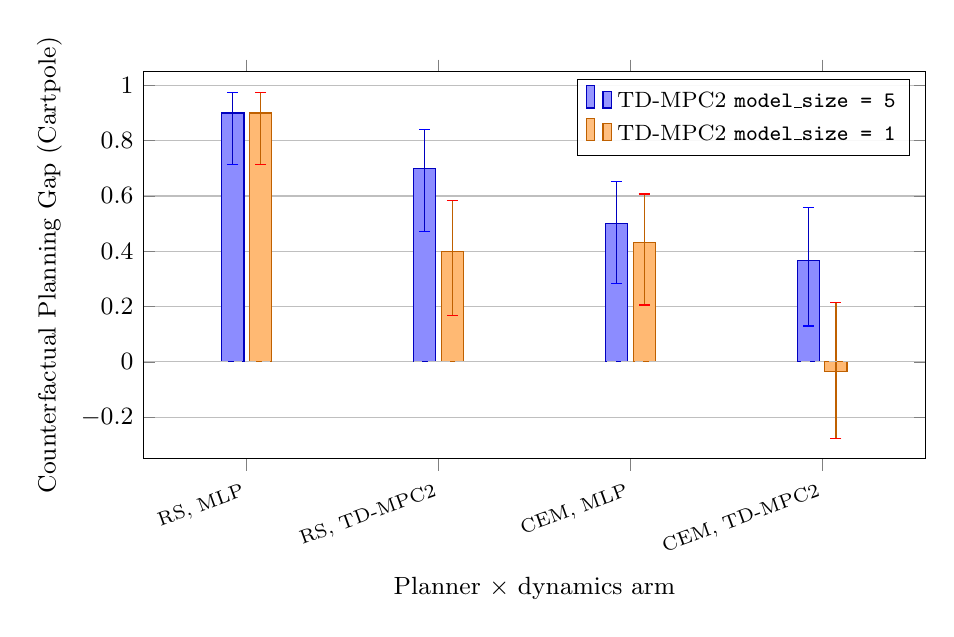
\begin{tikzpicture}
    \begin{axis}[
        width=0.95\columnwidth,
        height=6.5cm,
        font=\small,
        ybar=2pt,
        bar width=8pt,
        ymin=-0.35, ymax=1.05,
        ytick={-0.2, 0, 0.2, 0.4, 0.6, 0.8, 1.0},
        ylabel={Counterfactual Planning Gap (Cartpole)},
        ymajorgrids=true,
        xtick={1, 2, 3, 4},
        xticklabels={
          {RS, MLP},
          {RS, TD-MPC2},
          {CEM, MLP},
          {CEM, TD-MPC2},
        },
        x tick label style={font=\scriptsize, rotate=20, anchor=north east},
        xlabel={Planner $\times$ dynamics arm},
        legend cell align=left,
        legend style={
          at={(0.98, 0.98)}, anchor=north east,
          font=\footnotesize,
          fill=white, fill opacity=0.9, draw opacity=1, text opacity=1,
        },
        enlarge x limits=0.18,
      ]
      \addplot+[
          fill=blue!45, draw=blue!75!black,
          error bars/.cd, y dir=both, y explicit,
        ]
        table[x=x, y=y, y error plus=eplus, y error minus=eminus, row sep=\\] {
          x y     eplus eminus \\
          1 0.900 0.073 0.186  \\
          2 0.700 0.140 0.227  \\
          3 0.500 0.152 0.215  \\
          4 0.367 0.191 0.237  \\
        };
      \addlegendentry{TD-MPC2 \texttt{model\_size = 5}}
      \addplot+[
          fill=orange!55, draw=orange!75!black,
          error bars/.cd, y dir=both, y explicit,
        ]
        table[x=x, y=y, y error plus=eplus, y error minus=eminus, row sep=\\] {
          x y      eplus eminus \\
          1  0.900 0.073 0.186  \\
          2  0.400 0.183 0.233  \\
          3  0.433 0.174 0.227  \\
          4 -0.033 0.247 0.243  \\
        };
      \addlegendentry{TD-MPC2 \texttt{model\_size = 1}}
      \draw[densely dashed, gray!50] (axis cs:0.5, 0) -- (axis cs:4.5, 0);
    \end{axis}
  \end{tikzpicture}
  \caption{Cartpole capacity sweep at fixed $1 \times 10^{6}$-step training budget. Same four planner-dynamics combinations as Figure~\ref{fig:cross_env_cpg}, comparing TD-MPC2 \texttt{model\_size = 5} (blue) against \texttt{model\_size = 1} (orange), $n = 30$ pooled per bar with asymmetric AC error bars. The CEM~$\times$~TD-MPC2 cell at \texttt{model\_size = 1} (rightmost orange bar) is the only cell where the CI crosses zero: raw CPG $= -0.033$, AC CI $= [-0.28, +0.21]$, verdict \textsc{inconclusive}. Smaller-capacity TD-MPC2 closes the gap on Cartpole's CEM oracle that the larger-capacity model does not -- the metric reports this honestly rather than committing to a verdict the data does not support.}
  \label{fig:cartpole_capacity}
\end{figure}
